%-------------------------------------------------------------------------
% Section: our main work
%-------------------------------------------------------------------------

\chapter{Proposed solution }
\label{cha:proposed solution }
Now we can finally conclude why UIO driver doesn't work on some IPs with DMA, because AXI-Stream is a special bus protocol which is not compatible with AXI4 bus protocol. Figure~\ref{fig:Custom IP with AXI4-Lite/Full Register.} and Figure~\ref{fig:Custom IP with DMA and AXI-Stream Register.} show the difference of two designs. So, if we want to use UIO driver to control our custom AXI-Stream IP, we need to adapt UIO driver to control the DMA controller so that we can use it to submit DMA transaction to our IP.

We have modeled the high level problem and proposed a possible solution, but there is still some concerns. How do we submit DMA transaction through UIO? Is there any problem when doing the DMA transaction? 

\begin{figure}[!htb]
  \centering
  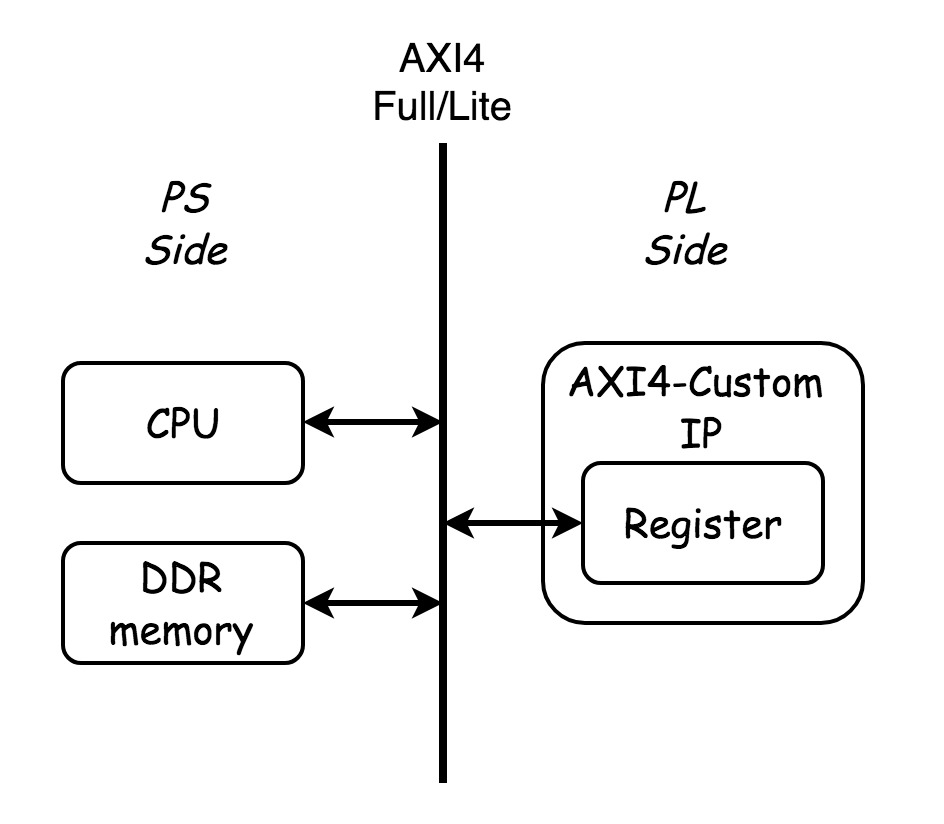
\includegraphics[scale=0.3]{images/customAXI4IP.jpg}
  \caption[Custom IP with AXI4-Lite/Full Register.]{Custom IP with AXI4-Lite/Full Register.}
  \label{fig:Custom IP with AXI4-Lite/Full Register.}
\end{figure}

\begin{figure}[!htb]
  \centering
  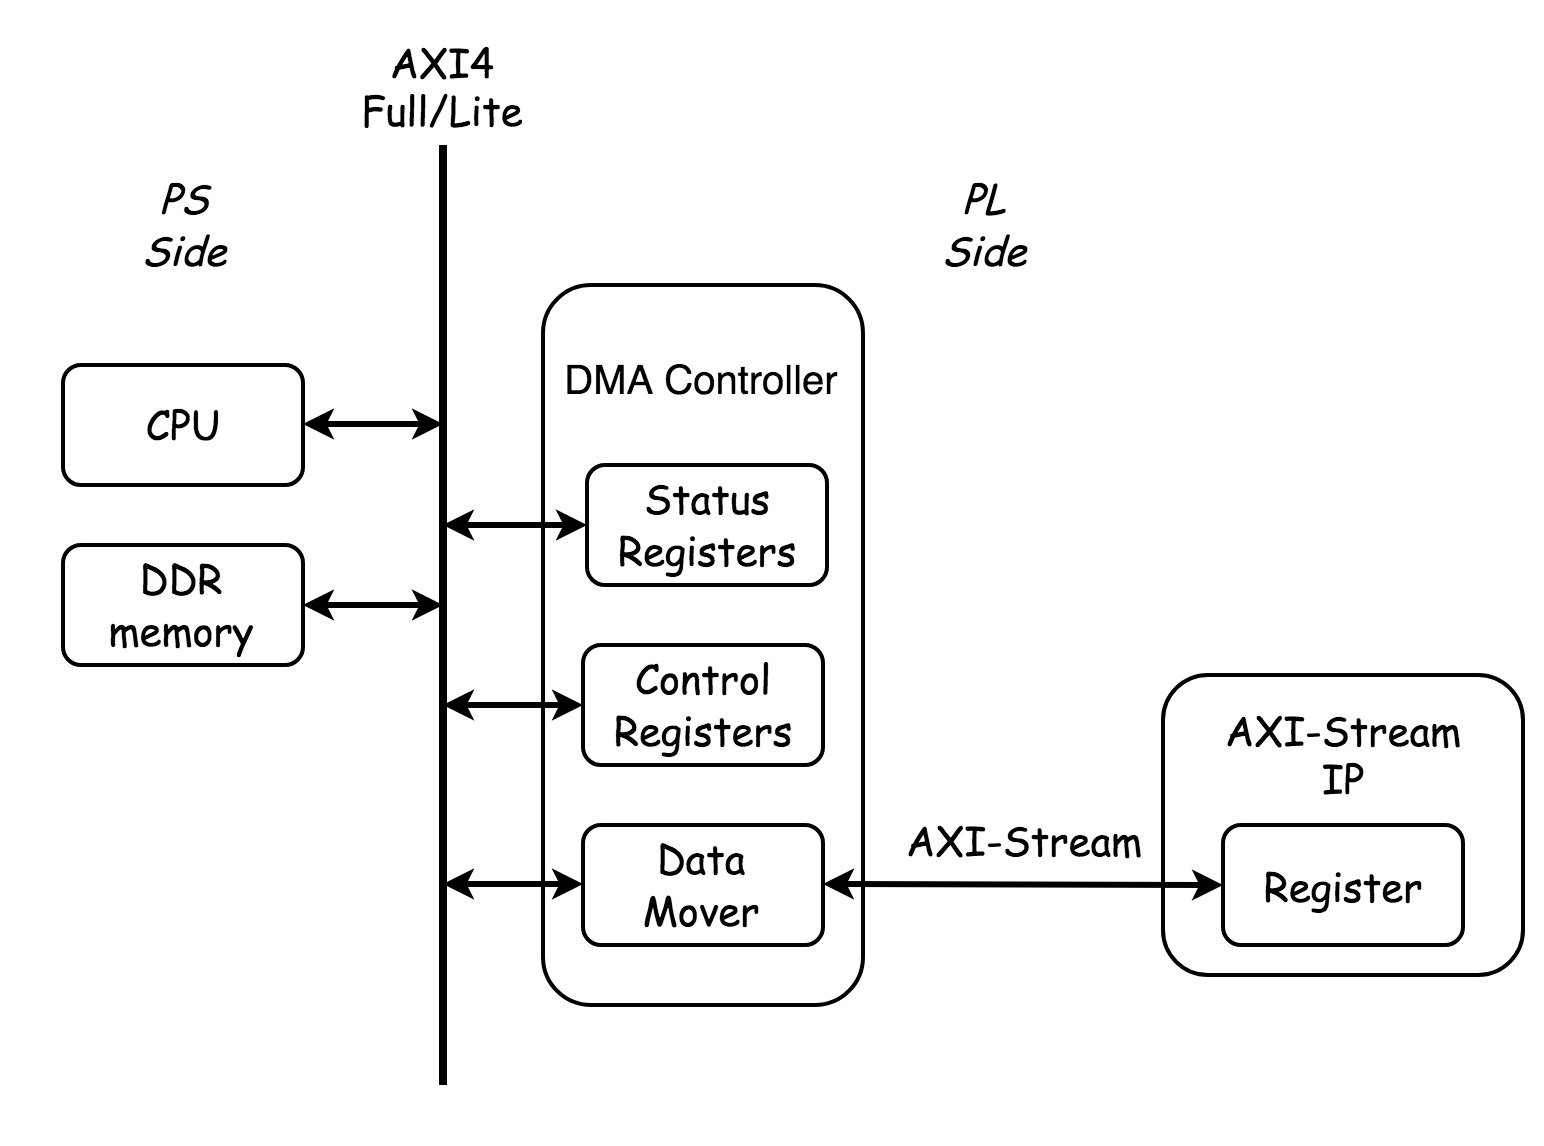
\includegraphics[scale=0.3]{images/customStreamIP.jpg}
  \caption[Custom IP with DMA and AXI-Stream Register.]{Custom IP with DMA and AXI-Stream Register.}
  \label{fig:Custom IP with DMA and AXI-Stream Register.}
\end{figure}
%-------------------------------------------------------------------------
% Section: 圖表
%-------------------------------------------------------------------------
\section{Problems}
\label{sec:Problems}

\subsection{File Operations.}
\label{subsec:File Operations}
Recall the normal usage of custom AXI4-Full/Lite IP with UIO,
\begin{lstlisting}[frame=single,language=C]
int main(void)
{
    int fd = open("/dev/uio0", O_RDWR);
    void *ptr = mmap(0, 0x10000, PROT_READ|PROT_WRITE, 
                     MAP_SHARED, fd, 0);
    volatile uint32_t *ctrl = (uint32_t *)ptr;
    *ctrl = 0x00000000;
    ...
}
\end{lstlisting}
typically, we open the device node to get device register pointer and memory-map to user memory, then we can manupulate the register like it is ..... The point is, we need file operations to communicate with DMA in UIO driver, 

Let's take a look at two file operations \textbf{write(), read()}. Figure~\ref{fig:UIO write andread functions.} shows what these two functions doing, basicly, these two functions in UIO driver is the handle about interrupt control. However, in our design, UIO node is actually a virtual device node, so interrupt control (and memory map) is no more needed. That means we can use \textbf{write(), read()} to do the \emph{\textbf{real}} read/write work.


\begin{figure}[!htb]
  \centering
  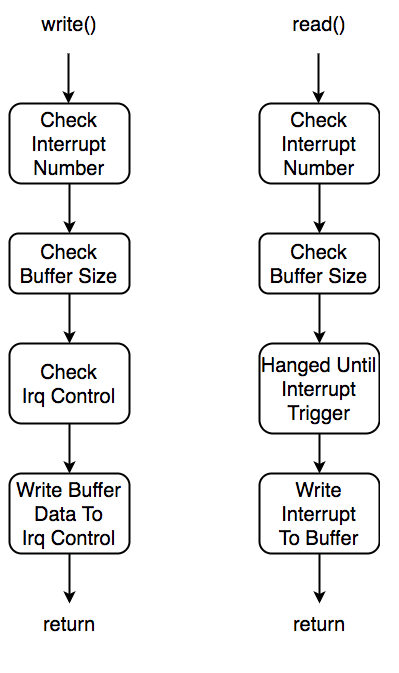
\includegraphics[scale=0.5]{images/uio_func_write.png}
  \caption[UIO write/read functions.]{UIO write/read functions}
  \label{fig:UIO write andread functions.}
\end{figure}

\subsection{Scatter Gather}
\label{subsec:Scatter Gather}
In tranditional DMA transaction, it can only accept a contiguous (nonsegmented) block of
physical memory, so, if we want to use DMA in userspace, and we can not get a contiguous 
memory space(like CMA), then we need to use DMA Scatter/Gather mode. This mode allows non-
contiguous (nonsegmented) block of physical memory and this mode need to be turn on in Vivado 
design first. In this mode, DMA controller automatically give the start address of the 
segmented of memory after the previous transaction of segmented memory is completed. To 
apply this mode, we need to construct a special data structure, Scatterlist, which collects 
start address and lengths of segmented block of user buffer memory. DMA engine will do the
transaction according to this list. 


\subsection{Cache Coherency}
\label{subsec:Cache Coherency}
While using DMA to do the data transfering, it may lead cache coherency problems. If we want to receive data to the buffer through the DMA, but the buffer is in cache now, to apply transaction, we give controller the buffer address and length. Once the transaction is done, we read the buffer and the value is same as old value. CPU think the value in memory is not changed because whole data transfering is through DMA controller, so CPU keeps the old buffer data in cache, that makes the difference between cache data and real data. Figure~\ref{fig:Cache Coherency Problems.} shows the cache coherency problem, both read and write may lead this problem, so if we want to transfer correct data, we must solve this problem.

\begin{figure}[!htb]
  \centering
  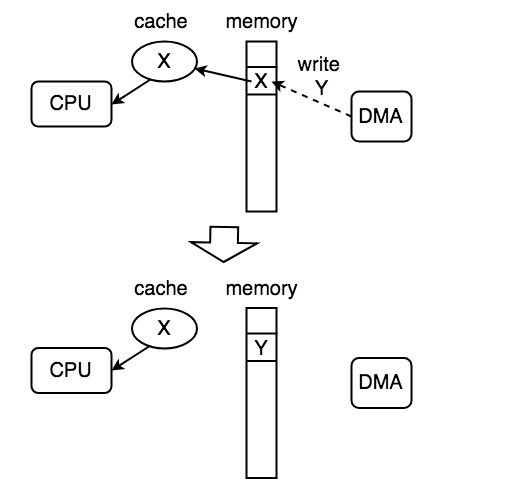
\includegraphics[scale=0.2]{images/cache_coherency.jpg}
  \caption[Cache Coherency Problems.]{Cache Coherency Problems.}
  \label{fig:Cache Coherency Problems.}
\end{figure}
%-------------------------------------------------------------------------
% Section: 圖表
%-------------------------------------------------------------------------
\section{Linux UIO driver for AXI DMA}
\label{sec:Linux UIO driver for AXI DMA}





\begin{figure}[!htb]
  \centering
  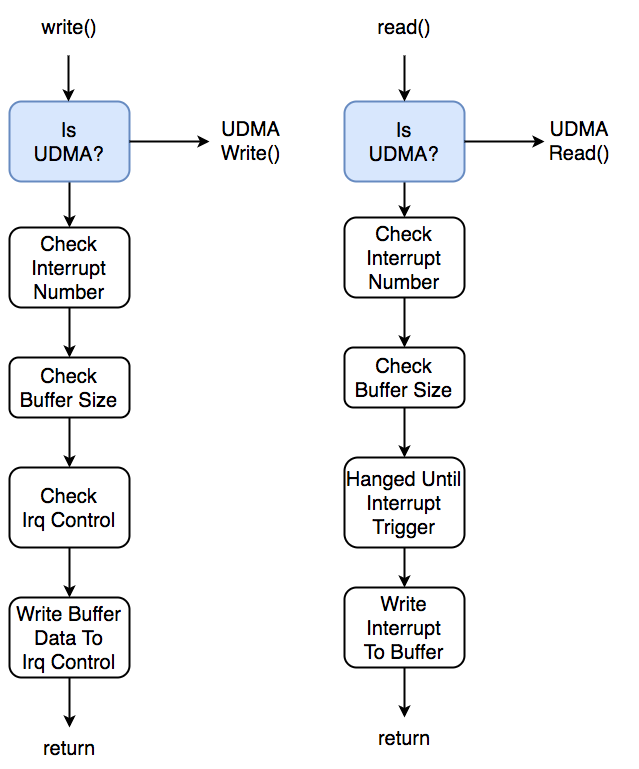
\includegraphics[scale=0.5]{images/udma_func_entry.png}
  \caption[UIO write/read functions.]{UIO write/read functions}
  \label{fig:UIO write andread functions.}
\end{figure}

\begin{figure}[!htb]
  \centering
  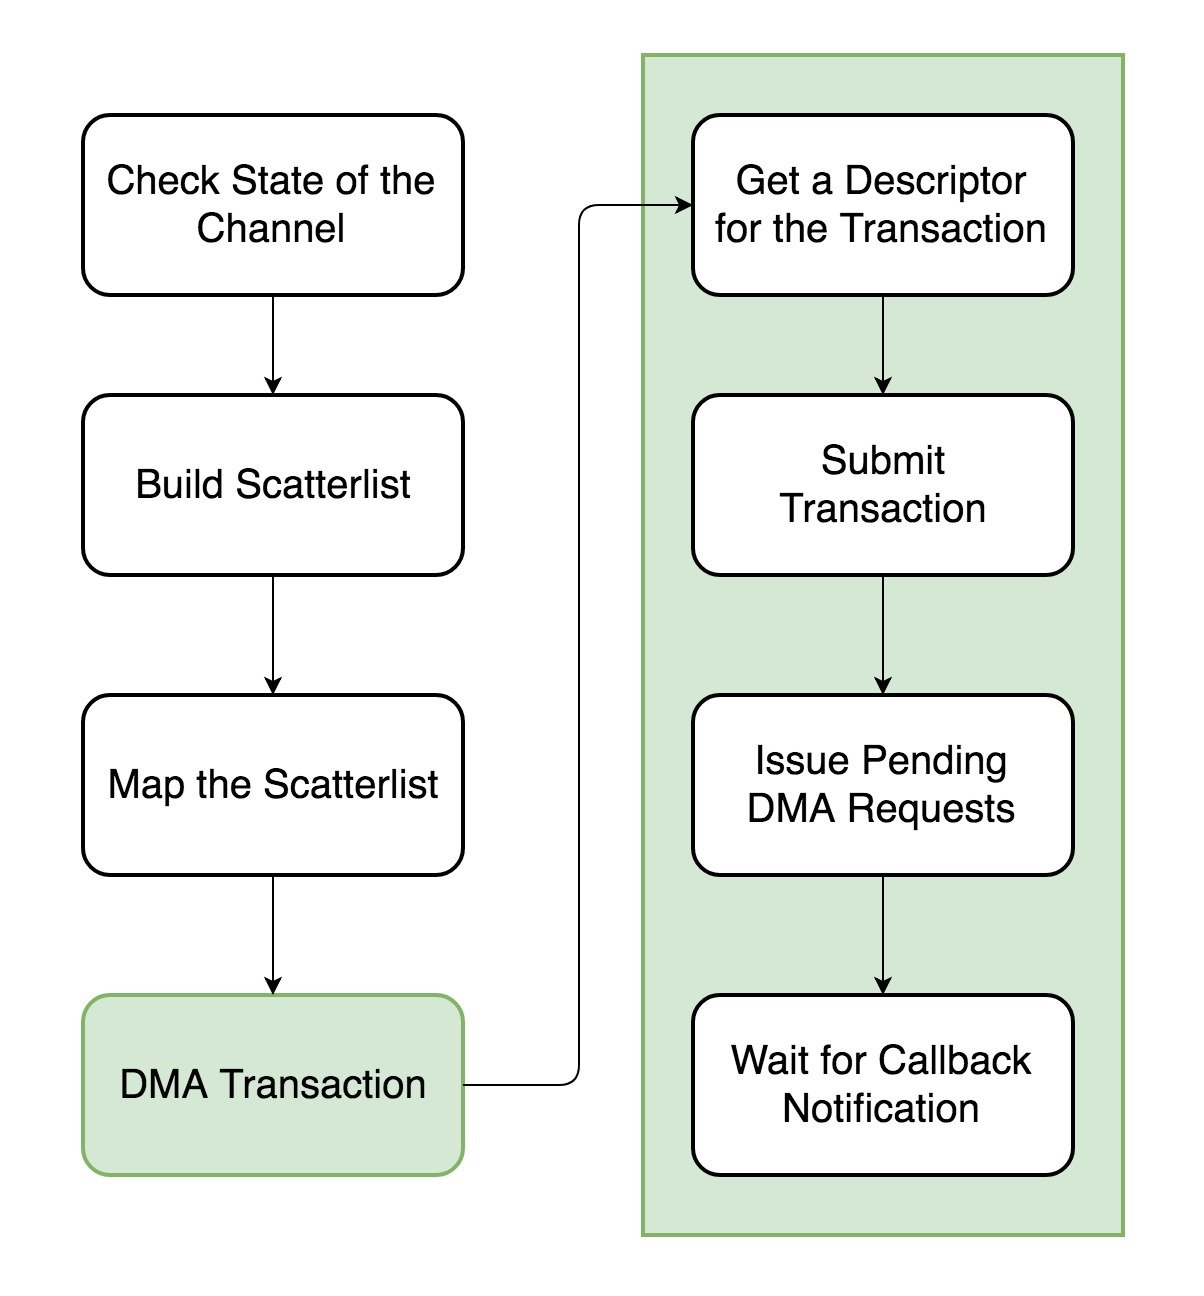
\includegraphics[scale=0.3]{images/udma_prepare_dma.jpg}
  \caption[Udma Prepare for DMA.]{udma prepare for dma.}
  \label{fig:Udma Prepare for DMA..}
\end{figure}



\begin{figure}[!htb]
  \centering
  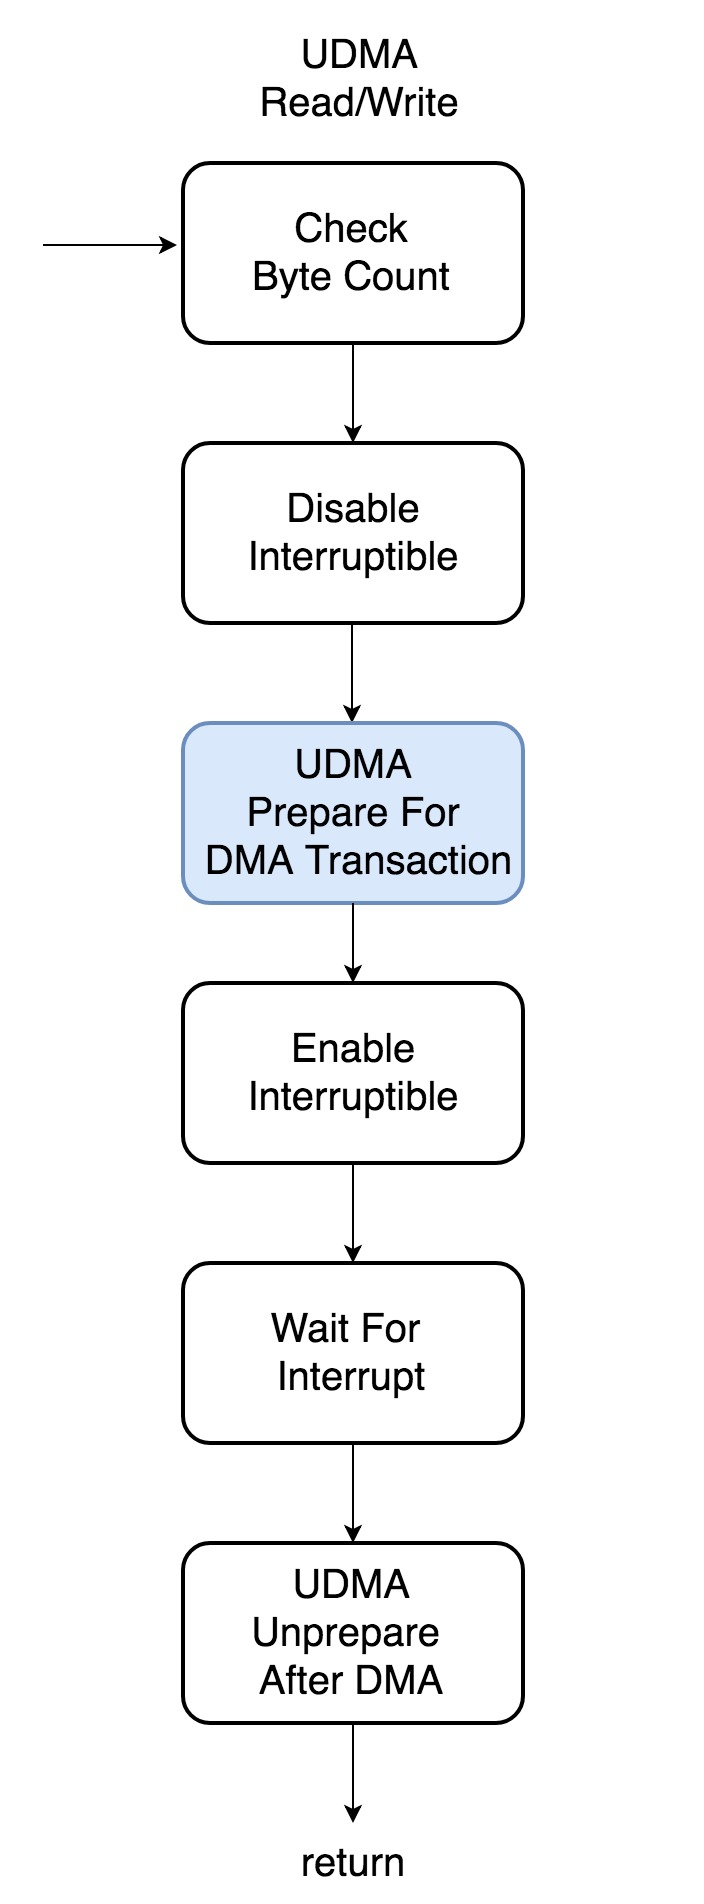
\includegraphics[scale=0.2]{images/udma_func.jpeg}
  \caption[UDMA write/read functions.]{UDMA write/read functions}
  \label{fig:UDMA write andread functions.}
\end{figure}

%-------------------------------------------------------------------------
% Section: Implementation
%-------------------------------------------------------------------------

\section{Implementation}
\label{sec:Implementation}

\subsection{Device Tree}
\label{subsec:Device Tree}
In first, we need to set our virtual device in our device tree file, in AXI4 IP, we have device block looks like:
\begin{lstlisting}[frame=single,language=C]
my_customIP@43c00000 {
	compatible = "generic-uio";
	reg = <0x43c00000 0x10000>;
	interrupts = <0 29 1>;
	interrupt-parent = <0x3>;
	xlnx,s00-axi-addr-width = <0x6>;
	xlnx,s00-axi-data-width = <0x20>;
};
\end{lstlisting}
It contains IP name, IP register address, register length, interrupt control...etc. These are essential properties if you want to apply a driver to control the device. But in our design, we have no real device, so the device tree will looks like:
\begin{lstlisting}[frame=single,language=C]
udma0 {
    compatible = "generic-uio";
    dmas = <dma-channel1 dma-channel2>;
    dma-names = "loop_tx", "loop_rx";   
    ezdma,dirs = <2 1>;                 
};
\end{lstlisting}
where dmas property refers to the DMA channel under ``axidma'' in device tree, for example, if ``axidma'' looks like:
\begin{lstlisting}[frame=single,language=C]
        loopback_dma: axidma@40410000 {
            #dma-cells = <1>;
            compatible = "xlnx,axi-dma";
            reg = < 0x40410000 0x10000 >;

            xlnx,include-sg;
            loopback_dma_mm2s_chan: dma-channel@40410000 {
                compatible = "xlnx,axi-dma-mm2s-channel";
                interrupt-parent = <&gic>;
                interrupts = <0 31 4>; 
                xlnx,datawidth = <0x20>;        
                xlnx,sg-length-width = <14>;    
                xlnx,device-id = <0x1>;     
            };

            loopback_dma_s2mm_chan: dma-channel@40410030 {
                compatible = "xlnx,axi-dma-s2mm-channel";
                interrupt-parent = <&gic>;
                interrupts = <0 32 4>;  
                xlnx,datawidth = <0x20>;       
                xlnx,sg-length-width = <14>;    
                xlnx,device-id = <0x1>;    
            };
        };
\end{lstlisting}
then ``dmas'' should be ``<\&loopback\_dma 0 \&loopback\_dma >'', dma-names is fixed in driver, please make sure the names are same as the setting. ``dirs'' tells driver the direction of DMA channel. If the direction is not same as declare in ``axidma'', it will fail when UIO is probing.After all these settings, our UIO driver should catch the device correctly and probe a device node under /dev.

\subsection{Compile New Kernel}
\label{subsec:Compile New Kernel}
Because we modified the UIO driver and add some new library, we need to compile a new kernel. First, replace the old ``uio.c'' and ``uio\_pdrv\_genirq.c'' with new files. Then put ``udma.c'' under ``drivers/uio'' folder, and ``udma.h'' under ``include/linux'' folder. We need to add ``obj-y\  += udma.o'' in Makefile under ``drivers/uio'' . After, we can compile our new kernel with new UIO driver which can support DMA functions.

\subsection{Linux On FPGA}
\label{subsec:Linux On FPGA}
Same as the we mentioned in former chapter, we boot Linux on FPGA in SD card with two partitions. The boot files in first partition have much changed in our scenario, ``devicetree.dtb'' and ``uImage'' we have discussed in former subsection. The modification in ``uEnv.txt'' is quite easy, this file provides additional environment variables for the bootloader,U-boot. It will looks like: 
\begin{lstlisting}[frame=single,language=C]
bootargs=console=ttyPS0,115200 root=/dev/mmcblk0p2 rootwait rw earlyprintk uio_pdrv_genirq.of_id=genric-uio
sdboot=if mmcinfo; then run uenvboot; echo Copying Linux from SD to RAM... && load mmc 0 ${kernel_load_address} ${kernel_image} && load mmc 0 ${devicetree_load_address} ${devicetree_image} && load mmc 0 ${ramdisk_load_address} ${ramdisk_image} && bootm ${kernel_load_address} - ${devicetree_load_address}; fi
\end{lstlisting}
To combine driver and device, please make sure the string behind ``uio\_pdrv\_genirq.of\_id=''(in this case, is ``generic-uio'') is same as the property ``compatible'' in device tree file.

\begin{figure}[!htb]
  \centering
  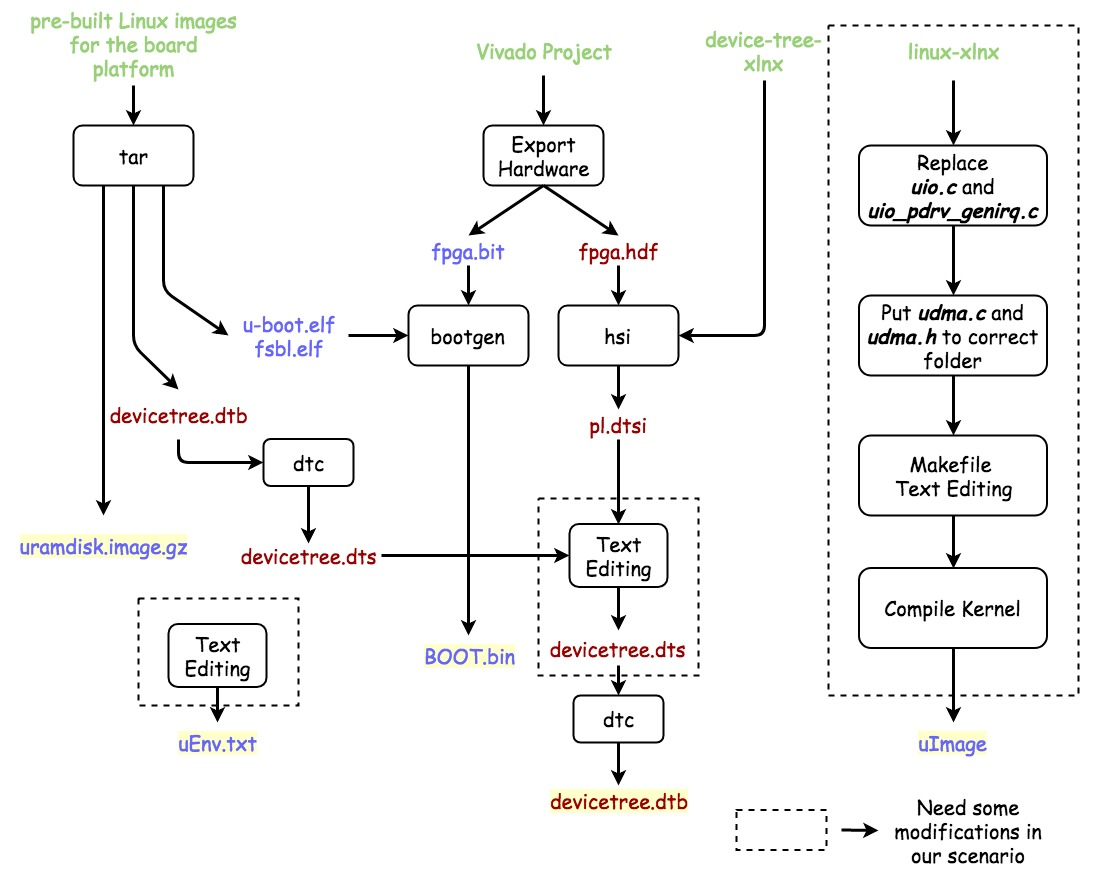
\includegraphics[scale=0.4]{images/new_embedded_linux.jpg}
  \caption[Embedded Linux on FPGA(UDMA ver.)]{Embedded Linux on FPGA(UDMA ver.)}
  \label{fig:Embedded Linux on FPGA(UDMA ver.)}
\end{figure}

Figure~\ref{fig:Embedded Linux on FPGA(UDMA ver.)} gives a simple illustration of our scenario.Unlike lots changes in first partition of SD card, we keep second partition as usual, this partition provides the file system when we boot our Linux, just keeps it as the same.

\subsection{Example}
\label{subsec:Example}

